\subsection{Application: Predictive Maintenance for Industrial Rotating Machinery}

Predictive maintenance is a foundational machine-learning application because the core challenge is not only fault prediction but also disciplined formulation of a rare-event classification problem from multivariate process measurements. Sensor values such as rotational speed, torque, temperature, and tool wear are continuous, correlated, and strongly affected by operating conditions. A useful model must therefore separate signal from operating-regime variation while avoiding leakage from identifiers, failure-mode labels, or information that would not be available at prediction time.

The application also illustrates why class imbalance and metric selection are central to practical machine learning. Machine failures are intentionally rare in a functioning industrial process, so accuracy can remain deceptively high even when a model fails to identify most breakdowns. Precision--recall analysis, threshold selection, and the cost of false alarms versus missed failures are therefore more informative than raw accuracy. These are the same validation and decision-theoretic ideas developed earlier in this chapter.

The quantitative experiment uses the UCI AI4I 2020 Predictive Maintenance dataset. The dataset is synthetic, but it was constructed to reflect common industrial predictive-maintenance variables and failure mechanisms. The goal here is not to claim production-level rotating-equipment performance; it is to provide a fully reproducible benchmark that demonstrates how feature preprocessing, class weighting, nonlinear models, and imbalance-aware evaluation affect a maintenance decision.

\textbf{Problem}

The task is to estimate the probability that a machine observation corresponds to a failure condition and to convert that probability into a maintenance alert. The learning objective must balance two competing errors: false negatives can allow a failure to go undetected, while false positives consume inspection capacity and may cause unnecessary downtime.

\textbf{Dataset}

The experiment uses the UCI AI4I 2020 Predictive Maintenance Dataset (UCI repository identifier 601). It contains 10,000 observations from a simulated milling-machine process and 339 positive machine-failure cases, corresponding to a failure prevalence of approximately 3.39\%. The predictive inputs include product type, air temperature, process temperature, rotational speed, torque, and tool wear. Identifier fields are excluded from the model. The benchmark uses a stratified 70/30 holdout split with random seed 1729 so that the rare positive class is represented in both training and evaluation partitions.

\textbf{Model}

Three conventional supervised-learning baselines are compared under the same split. Standard logistic regression provides a linear probabilistic baseline. Balanced logistic regression applies class weighting to change the optimization objective under the rare-event distribution. A class-balanced random forest supplies a nonlinear baseline that can model interactions among torque, speed, temperature, and wear without requiring a specialized deep architecture.

\textbf{Method}

Numerical variables are standardized using statistics learned from the training partition for the logistic models, while the categorical product type is one-hot encoded. The random forest receives the same feature set with the categorical variable encoded consistently. All models are evaluated on the identical held-out partition. Average precision and ROC--AUC measure ranking quality, and a precision--recall sweep identifies the threshold with the strongest F1 score for this controlled comparison.

\textbf{Evaluation}

Figure~\ref{fig:ch1-predictive-maintenance-ai4i} combines a feature-space diagnostic with the imbalance-aware model comparison. Panel (a) plots torque against rotational speed for a deterministic subset of normal observations together with all failure observations, showing that failure cases occupy overlapping rather than trivially separable regions of the operating space. Panel (b) reports precision--recall curves for the three models and includes the held-out failure prevalence as the no-skill reference. Table~\ref{tab:ch1-predictive-maintenance-benchmark} provides the reproduced numerical comparison.

\begin{figure}[t]
\centering
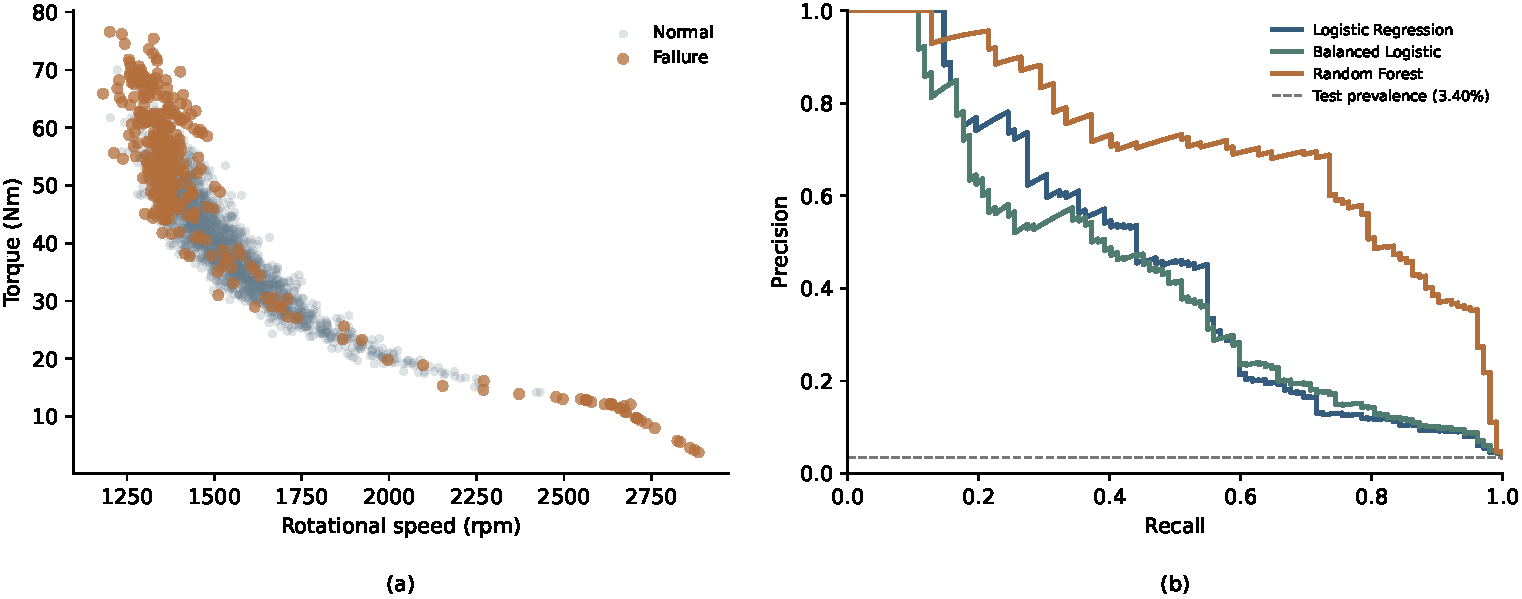
\includegraphics[width=\BookFigureWidth]{figures/ch01_predictive_maintenance_ai4i.pdf}
\caption{Reproduced predictive-maintenance diagnostics on the UCI AI4I 2020 dataset. (a) Torque versus rotational speed for a deterministic subset of normal observations and all observed failure cases. Failures overlap the normal operating region, illustrating why a single scalar rule is insufficient for reliable detection. (b) Precision--recall curves for standard logistic regression, class-balanced logistic regression, and a class-balanced random forest on the same stratified holdout split. The dashed horizontal line marks the test-set failure prevalence, providing the appropriate rare-event baseline for interpreting precision.}
\label{fig:ch1-predictive-maintenance-ai4i}
\end{figure}

\begin{table}[t]
\centering
\small
\caption{Reproduced model comparison on the UCI AI4I 2020 Predictive Maintenance Dataset. AP denotes average precision. Precision, recall, and F1 are reported at the F1-maximizing threshold for the controlled holdout comparison.}
\label{tab:ch1-predictive-maintenance-benchmark}
\begin{tabular}{lrrrrr}
\toprule
Model & AP & ROC--AUC & F1 & Precision & Recall \\
\midrule
Logistic regression & 0.4583 & 0.8939 & 0.4956 & 0.4516 & 0.5490 \\
Balanced logistic & 0.4295 & 0.9039 & 0.4623 & 0.4742 & 0.4510 \\
Random forest & 0.7109 & 0.9764 & 0.7109 & 0.6881 & 0.7353 \\
\bottomrule
\end{tabular}
\end{table}

\textbf{Results}

The nonlinear random-forest baseline produces the strongest rare-event discrimination in this controlled experiment, with average precision of 0.7109, ROC--AUC of 0.9764, and F1 of 0.7109. Standard logistic regression achieves average precision of 0.4583, while class weighting improves ROC--AUC slightly but does not improve average precision or F1 under this split. The comparison demonstrates that class weighting is not automatically beneficial: it changes the optimization objective, but the resulting thresholded operating point must still be validated empirically.

\textbf{Error Analysis}

The precision--recall curves show that the dominant challenge is separating failures from a large population of normal observations with overlapping sensor values. False negatives should be analyzed by failure mechanism and operating region, while false positives should be examined for combinations of high torque, atypical rotational speed, elevated temperatures, or large tool wear that resemble failure conditions without crossing the true failure criteria. Error analysis should also test whether performance varies systematically by product type.

\textbf{Limitations}

AI4I is synthetic rather than a direct record of fielded rotating machinery, so the benchmark cannot establish deployment performance for a specific industrial asset. The random holdout also does not model temporal drift, machine-to-machine domain shift, maintenance interventions, or repeated measurements from the same physical asset. A production study should use asset-level or time-ordered partitioning on real sensor histories and should report uncertainty across multiple machines and operating conditions.

\textbf{Deployment / Engineering Implications}

The Chapter 1 lesson is that a predictive-maintenance model is only one component of a decision process. Deployment requires a threshold tied to inspection cost and failure risk, monitoring for changes in failure prevalence and operating conditions, and periodic recalibration. A model with strong ROC--AUC can still be operationally poor if its precision at the maintenance threshold is inadequate, so the validation metric must be chosen to match the engineering decision rather than the convenience of the model.
